\section{Results}
\label{sec:7}

All results are reported on the Application population ($V_{\text{app}}$) against the primary oracle $I^*(v)$, under the input--label independence guarantee (Section~\ref{sec:4.4}). Per-fold results, secondary strata and extended protocol notes are in the Supplementary Material and the experiment pages of the replication repository (Section~\ref{sec:6.1}). Figure~\ref{fig:results} summarizes the three main findings.

\begin{figure}[htbp]
\centering
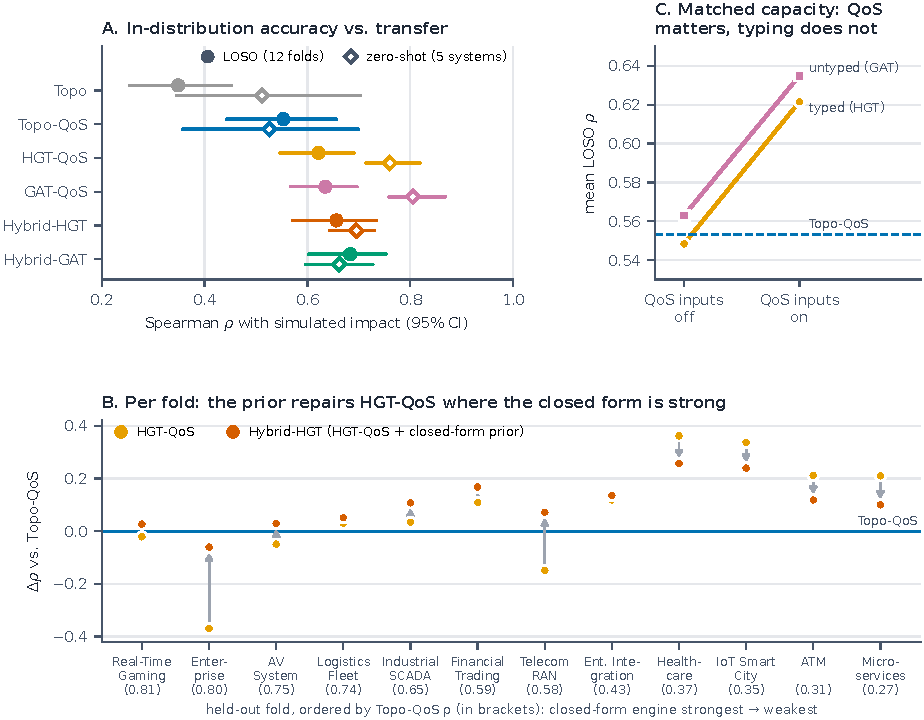
\includegraphics[width=\linewidth]{figures/Figure_5}
\caption{Main results at a glance, Application population. (A)~Mean Spearman $\rho$ with 95\% bootstrap intervals under LOSO (filled circles; CPU sweeps of Table~\ref{tab:hybrid}) and zero-shot on the five system models (open diamonds). The hybrids lead on unseen synthetic architectures; the pure learned engines transfer best. (B)~Per held-out fold, the gain of \texttt{HGT-QoS} and of Hybrid-HGT over \texttt{Topo-QoS}; the arrow shows what the closed-form prior changes. It removes the learned engine's losses where the closed-form engine is strongest (Enterprise, Telecom RAN) and trims its largest gains where it is weakest. (C)~Cell means of the capacity- and channel-matched $2\times2$ (Table~\ref{tab:contrasts_matched}): QoS inputs raise both models by about $0.07$, a gain Section~\ref{sec:rq2} traces to three node features rather than the edge channel, while the typed and untyped lines stay together.}
\label{fig:results}
\end{figure}

\subsection{RQ1: SaG's Engines Against Structural Baselines}
\label{sec:rq1}
\label{sec:rq1-loso}

\paragraph{Summary} \emph{SaG's QoS-weighted closed-form engine (\texttt{Topo-QoS}, $\rho = 0.553$) outperforms unweighted centrality ($\rho = 0.349$) on all twelve held-out architectures ($+0.204$, $p = 0.0005$). On their own, the learned engines are statistically on par with it (\texttt{HGT-QoS} $0.622$, \texttt{GAT-QoS} $0.635$). The hybrid engines, in which a learned engine corrects the closed-form score, significantly outperform it ($+0.103$ and $+0.130$, each on 11/12 folds, Holm $p \le 0.0068$).}

Each of the twelve folds holds out one scenario and trains on the remaining eleven, and every predictor is scored on the same Application node set (26 to 300 nodes, $K$ between 5 and 60). Table~\ref{tab:hybrid} reports SaG's six engines and baselines from one family of CPU runs, in which the shared comparator rows are bit-identical.

\begin{table}[htbp]
\centering
\small
\caption{Main results. SaG's engines against the structural baselines under LOSO (twelve synthetic architectures, five seeds, Application population, CPU runs) and zero-shot on the five open-source system models (protocol of Table~\ref{tab:9b}). $\Delta\rho$ is paired by fold against the registered comparator \texttt{Topo-QoS}, with a bootstrap 95\% CI ($B = 2{,}000$) and a two-sided Wilcoxon test. $p_{\text{Holm}}$ is given for the hybrids, within each one's registered family (vs.\ \texttt{Topo-QoS} and vs.\ its own learned engine). The registered GPU sweep of \texttt{HGT-QoS}: Supplementary Section~\ref{S-supp:loso-gpu}. Per-fold values: Supplementary Section~\ref{S-supp:hybrid-folds}.}
\label{tab:hybrid}
\resizebox{\linewidth}{!}{%
\begin{tabular}{lccccccc}
\toprule
 & \multicolumn{5}{c}{\textbf{LOSO, twelve synthetic architectures}} & \multicolumn{2}{c}{\textbf{Five system models}} \\
\cmidrule(lr){2-6}\cmidrule(lr){7-8}
\textbf{Predictor} & \textbf{Mean $\rho$ [95\% CI]} & \textbf{$\Delta\rho$ vs \texttt{Topo-QoS} [95\% CI]} & \textbf{Won} & \textbf{$p$ ($p_{\text{Holm}}$)} & \textbf{Overlap@$K$} & \textbf{$\rho$ [95\% CI]} & \textbf{PR-AUC} \\
\midrule
\textbf{Topo} & 0.349 $[0.254, 0.452]$ & $-0.204$ $[-0.286, -0.122]$ & 0/12 & 0.0005 & 0.366 & 0.511 $[0.346, 0.703]$ & 0.474 \\
\textbf{Topo-QoS} & 0.553 $[0.443, 0.657]$ & --- & --- & --- & 0.388 & 0.526 $[0.357, 0.699]$ & 0.474 \\
\textbf{HGT-QoS} & 0.622 $[0.547, 0.690]$ & $+0.069$ $[-0.046, +0.174]$ & 8/12 & 0.266 & 0.426 & 0.760 $[0.714, 0.819]$ & 0.713 \\
\textbf{GAT-QoS} & 0.635 $[0.567, 0.696]$ & $+0.082$ $[-0.046, +0.201]$ & 7/12 & 0.233 & 0.438 & \textbf{0.805} $[0.759, 0.868]$ & \textbf{0.790} \\
\textbf{Hybrid-HGT} & 0.657 $[0.572, 0.733]$ & $+0.103$ $[+0.055, +0.152]$ & 11/12 & 0.0034 (0.0068) & 0.435 & 0.695 $[0.643, 0.730]$ & 0.602 \\
\textbf{Hybrid-GAT} & \textbf{0.683} $[0.603, 0.753]$ & $\mathbf{+0.130}$ $[+0.075, +0.190]$ & \textbf{11/12} & \textbf{0.0015} (\textbf{0.0029}) & \textbf{0.450} & 0.662 $[0.597, 0.727]$ & 0.600 \\
\bottomrule
\end{tabular}%
}
\end{table}

\noindent\textbf{The QoS-aware projection is the largest single gain.} Re-weighting shortest paths by declared QoS contracts lifts closed-form ranking from $\rho = 0.349$ to $0.553$ on every held-out architecture. Every learned model reads centralities computed on the same QoS-weighted projection (Section~\ref{sec:3.4}), and a regressor on those per-component features alone reaches $\rho = 0.642$ (Section~\ref{sec:rq2}), so the representation carries much of the signal the learned engines use.

\noindent\textbf{On their own, learned engines are on par with the closed-form engine.} \texttt{HGT-QoS} ($+0.069$, $p = 0.266$) and \texttt{GAT-QoS} ($+0.082$, $p = 0.233$) lead \texttt{Topo-QoS} numerically, with intervals spanning zero. The registered confirmatory contrast, run on the GPU sweep the plan specified, agrees ($+0.085$, $p = 0.151$, Holm $0.303$; Supplementary Section~\ref{S-supp:loso-gpu}).

\noindent\textbf{Both hybrids significantly outperform the closed-form engine.} Hybrid-HGT reaches $\rho = 0.657$ ($+0.103$, Holm $p = 0.0068$) and Hybrid-GAT reaches $\rho = 0.683$ ($+0.130$, CI $[+0.075, +0.190]$, Holm $p = 0.0029$), each on 11 of 12 folds. Each meets the decision rule registered before its run. Both remain significant under one Holm correction pooled over all thirteen registered contrasts of the study ($p_{\text{omni}} = 0.041$ and $0.019$; Section~\ref{sec:6.3}). They are the only models in this study that significantly beat closed-form ranking: the feature-only regressor of Section~\ref{sec:rq2} does not ($+0.089$, $p = 0.176$). Among the engines of Table~\ref{tab:hybrid}, Hybrid-GAT has the highest Overlap@$K$ ($0.450$); the feature-only regressors reach $0.455$--$0.471$.

\noindent\textbf{Why the hybrids work: the engines are complementary.} \texttt{HGT-QoS} loses to \texttt{Topo-QoS} on four folds, all where the closed-form engine is strongest: Real-Time Gaming, Enterprise ($0.426$ vs.\ $0.795$), AV System and Telecom RAN ($0.427$ vs.\ $0.576$). Its largest gains come where the closed-form engine is weakest: Healthcare, IoT Smart City, ATM and Microservices, $+0.210$ to $+0.362$ (Figure~\ref{fig:results}B). The prior removes the failure mode: on Enterprise, Hybrid-HGT and Hybrid-GAT reach $0.735$ and $0.768$, and Telecom RAN turns from a loss into a win for both. The cost is a smaller gain on the weakest folds.

\noindent\textbf{Anchoring trades transfer for in-distribution accuracy.} On the five independently authored system models, both hybrids stay well above every training-free score ($0.695$ and $0.662$ vs.\ $0.511$--$0.526$) but below the pure learned engines ($0.760$ and $0.805$; Section~\ref{sec:rq3}). By the rule registered in Amendment~6, Hybrid-GAT therefore does not replace Hybrid-HGT as the recommended hybrid ($0.662 < 0.695$).

\noindent\textbf{Label noise and inert components.} Re-running the oracle across five seeds gives a test--retest rank correlation of $0.811$--$1.000$ (median $0.982$), well above every engine's mean $\rho$. Between $21\%$ and $52\%$ of each held-out population carries zero simulated impact. In the registered sweep, restricting evaluation to components with positive impact halves every predictor's correlation, learned or not, and leaves the method ordering unchanged (Supplementary Section~\ref{S-supp:loso-active}).

\subsubsection{How the Hybrids Are Built}
\label{sec:rq1-hybrid}

Each hybrid gives a learned engine the rank-normalized \texttt{Topo-QoS} score as one extra input per Application and Library, and adds a learned correction to that score on the logit scale, $\hat{I}^*(v) = \sigma\big(z(v) + \alpha\,\operatorname{logit}(p(v))\big)$, with one learnable $\alpha$ (Figure~\ref{fig:engines}a). Everything else matches the underlying engine. Hybrid-HGT is built on \texttt{HGT-QoS} (Amendment~5; $321$ extra parameters) and Hybrid-GAT on \texttt{GAT-QoS} (Amendment~6; $1{,}441$ extra parameters). Each was registered with its contrasts and decision rule before any run, with no setting tuned, and evaluated in its own CPU sweep with its comparators re-run in the same invocation.

\subsection{RQ2: What Learned Engines Need}
\label{sec:rq2}

\paragraph{Summary} \emph{At matched capacity, relation-specific weights add nothing (typing main effect $-0.014$), and neither does message passing: a gradient-boosted regressor that reads the same per-component features and has no graph model matches the learned engines ($\rho = 0.642$, against $0.635$ for \texttt{GAT-QoS} and $0.622$ for \texttt{HGT-QoS}). The untyped engine's QoS gain ($+0.072$) is carried by three declared-coupling node features ($+0.095$, 11 of 12 folds), not by the 16-D edge channel ($-0.023$). The registered directionality control confirms it for the typed engine: without its reverse pass, HGT receives no messages at Applications and loses nothing ($\rho = 0.632$ against $0.622$, $p = 0.91$).}

A first comparison against small untyped GATs ($28{,}168$ parameters against HGT's $434{,}620$, reading at most a scalar edge weight) credited typing with a large gain ($+0.234$ without QoS). That gain is an effect of capacity and channel width (Supplementary Sections~\ref{S-supp:naive-2x2} and~\ref{S-supp:loso-gpu}), and the control registered in Amendment~2 removes both differences. \texttt{GAT} and \texttt{GAT-QoS} are untyped GATs at HGT's parameter budget ($437{,}496$ and $429{,}992$), and \texttt{GAT-QoS} reads the same 16-D edge vector as \texttt{HGT-QoS}, including the relation one-hot. All four matched arms ran in one CPU sweep, and the decision rule was fixed before any control result existed (Table~\ref{tab:contrasts_matched}).

\begin{table}[htbp]
\centering
\small
\caption{The $2\times2$ with capacity and edge-channel width matched (Amendment~2): \texttt{GAT} ($\neg$T$\neg$Q, $437{,}496$ parameters), \texttt{HGT} (T$\neg$Q, $434{,}620$), \texttt{GAT-QoS} ($\neg$TQ, $429{,}992$), \texttt{HGT-QoS} (TQ, $434{,}620$). One CPU sweep, twelve LOSO folds, five seeds, Application population. Holm correction across the three orthogonal quantities; simple effects are descriptive. Cell means: $0.563$, $0.548$, $0.635$, $0.622$. The Q factor switches the 16-D edge channel and the three QoS node columns together; Table~\ref{tab:attribution} separates them.}
\label{tab:contrasts_matched}
\resizebox{\linewidth}{!}{%
\begin{tabular}{llrccccl}
\toprule
\textbf{Quantity} & \textbf{Contrast} & \textbf{$\Delta\rho$} & \textbf{95\% CI} & \textbf{Won} & \textbf{$W$} & \textbf{$p$} & \textbf{$p_{\text{Holm}}$} \\
\midrule
\multicolumn{8}{l}{\textit{Three orthogonal quantities, Holm-corrected across these three}} \\
\textbf{Typing (main effect)} & averaged over Q & $-0.014$ & $[-0.052, +0.023]$ & 4/12 & 29.0 & 0.470 & 0.940 \\
\textbf{QoS inputs (main effect)} & averaged over T & $\mathbf{+0.073}$ & $[+0.013, +0.120]$ & 10/12 & 13.0 & 0.043 & 0.127 \\
\textbf{Typing $\times$ QoS interaction} & difference of differences & $+0.001$ & $[-0.050, +0.042]$ & 6/12 & 34.0 & 0.733 & 0.940 \\
\midrule
\multicolumn{8}{l}{\textit{Simple effects --- descriptive, not separately corrected}} \\
\textbf{Typing, QoS absent} & HGT vs.\ GAT & $-0.015$ & $[-0.064, +0.033]$ & 5/12 & 31.0 & 0.569 & --- \\
\textbf{Typing, QoS present} & HGT-QoS vs.\ GAT-QoS & $-0.013$ & $[-0.054, +0.026]$ & 4/12 & 27.0 & 0.380 & --- \\
\textbf{QoS inputs, typing absent} & GAT-QoS vs.\ GAT & $\mathbf{+0.072}$ & $[+0.028, +0.109]$ & 10/12 & 9.0 & 0.016 & --- \\
\textbf{QoS inputs, typing present} & HGT-QoS vs.\ HGT & $+0.073$ & $[-0.002, +0.136]$ & 10/12 & 19.0 & 0.129 & --- \\
\bottomrule
\end{tabular}%
}
\end{table}

\noindent\textbf{Relation-specific weights add nothing once capacity is matched.} \texttt{HGT} and \texttt{HGT-QoS} are within $0.015$ of their untyped counterparts \texttt{GAT} and \texttt{GAT-QoS} and win only 4--5 of 12 folds against them. The untyped arms, however, receive no messages at the Applications they score (Section~\ref{sec:6.2}). The registered $2\times2$ therefore compares typed message passing with per-component learning, not two message-passing architectures, and Table~\ref{tab:attribution} asks what each of its ingredients contributes.

\begin{table}[htbp]
\centering
\small
\caption{Attribution controls (exploratory; Amendment~7). One CPU sweep, twelve LOSO folds, five seeds, Application population, with \texttt{GAT} and \texttt{GAT-QoS} re-run in the same invocation (bit-identical to Table~\ref{tab:contrasts_matched}). \texttt{GAT-QoS-nf} is \texttt{GAT-QoS} reading \texttt{GAT}'s node features; each of its inputs is bit-identical to one parent arm. \texttt{GBM-Feat}(-\texttt{QoS}) is gradient boosting on \texttt{GAT}'s (\texttt{GAT-QoS}'s) node features. Holm correction across the five contrasts. Cell means: \texttt{GBM-Feat} $0.642$, \texttt{GBM-Feat-QoS} $0.632$, \texttt{GAT-QoS-nf} $0.540$. Per-fold values: Supplementary Section~\ref{S-supp:attribution}.}
\label{tab:attribution}
\resizebox{\linewidth}{!}{%
\begin{tabular}{llrccccl}
\toprule
\textbf{Quantity} & \textbf{Contrast} & \textbf{$\Delta\rho$} & \textbf{95\% CI} & \textbf{Won} & \textbf{$W$} & \textbf{$p$} & \textbf{$p_{\text{Holm}}$} \\
\midrule
\textbf{QoS node columns, edge channel held} & GAT-QoS vs.\ GAT-QoS-nf & $\mathbf{+0.095}$ & $[+0.048, +0.135]$ & 11/12 & 5.0 & 0.0049 & 0.024 \\
\textbf{QoS edge channel, node features held} & GAT-QoS-nf vs.\ GAT & $-0.023$ & $[-0.046, -0.004]$ & 3/12 & 15.0 & 0.064 & 0.192 \\
\textbf{QoS node columns, no graph model} & GBM-Feat-QoS vs.\ GBM-Feat & $-0.010$ & $[-0.028, +0.006]$ & 5/12 & 30.0 & 0.519 & 1.000 \\
\textbf{Neural vs.\ trees, QoS-off features} & GAT vs.\ GBM-Feat & $-0.079$ & $[-0.134, -0.028]$ & 1/12 & 7.0 & 0.0093 & 0.037 \\
\textbf{Neural vs.\ trees, QoS-on features} & GAT-QoS vs.\ GBM-Feat-QoS & $+0.003$ & $[-0.048, +0.054]$ & 7/12 & 39.0 & 1.000 & 1.000 \\
\bottomrule
\end{tabular}%
}
\end{table}

\noindent\textbf{The QoS gain is carried by three node features, not the edge channel.} The Q factor of Table~\ref{tab:contrasts_matched} switches two inputs together: the 16-D edge vector and three node columns holding each component's declared coupling weights ($w$, $w_{\text{in}}$, $w_{\text{out}}$; Section~\ref{sec:3.4}). Removing the three columns from \texttt{GAT-QoS} costs $0.095$ (11 of 12 folds, Holm $p = 0.024$), while adding the edge channel to \texttt{GAT} changes nothing ($-0.023$, 3 of 12). The training stabilization the channel appeared to provide follows the same columns: the median within-fold seed spread is $0.010$ for \texttt{GAT-QoS}, $0.083$ for \texttt{GAT} and $0.136$ for \texttt{GAT-QoS-nf}. The architecture explains this: no edge reaches an Application in the untyped engines, so the channel can affect Application scores only indirectly, through weights shared with other entity types during training.

\noindent\textbf{Message passing adds nothing measurable on this target.} The untyped engines score each Application from its own features, and the typed HGT, which aggregates over $35$--$59\%$ of the graph, does not outperform them. The directionality control registered in Amendment~2, run after Amendment~7, tests this within HGT: removing the reverse pass removes every message into an Application, and \texttt{HGT-QoS-U} ($330{,}895$ parameters) reaches $\rho = 0.632$ $[0.570, 0.687]$ against $0.622$ for \texttt{HGT-QoS} ($-0.010$ for \texttt{HGT-QoS}, 6 of 12 folds, $p = 0.91$; Supplementary Section~\ref{S-supp:attribution}). Its median seed spread also falls, from $0.056$ to $0.020$. The capacity control registered with it answers from the untyped side: \texttt{GAT-w}, an untyped GAT at HGT's parameter budget ($439{,}272$) reading the same QoS node features and a scalar edge weight, reaches $0.633$ ($-0.011$ for \texttt{HGT-QoS}, 5 of 12 folds, $p = 0.68$) and is level with \texttt{GAT-QoS} ($-0.002$), so the width of an edge channel that never reaches an Application is immaterial. The feature-only regressor, \texttt{GBM-Feat} (declared in Amendment~3), reads the identical feature tensors with no graph model and reaches $\rho = 0.642$ $[0.547, 0.725]$. That is on par with \texttt{GAT-QoS} ($+0.003$ for the matched-feature pair) and with \texttt{HGT-QoS} ($+0.021$, 7 of 12 folds, paired across sweeps whose shared arms are bit-identical). The three QoS columns do not help the regressor ($-0.010$). The neural model needs them to reach what the trees extract from the QoS-weighted centralities: without them, \texttt{GAT} trails \texttt{GBM-Feat} on 11 of 12 folds ($-0.079$). The learned engines' margin over closed-form ranking is therefore the learned combination of SaG's per-component features, not aggregation over the graph. Only the hybrids, which add the closed-form score to those features, significantly beat closed-form ranking (Section~\ref{sec:rq1}).

\noindent\textbf{How much the target can reward.} $I^*(v)$ is a near-topological target: a topology-only relabeling recovers its ordering at mean $\rho = 0.965$, and QoS acts mainly at its top-$K$ boundary (Section~\ref{sec:4.3}). The learned models reach QoS through the QoS-weighted centralities and declared coupling weights among their node features, and on this target the edge encodings contribute nothing measurable. Two things are needed before either the encodings or message passing can be credited with contract semantics: oracles that express deadline misses, durability replay or priority inversion, and a substrate on which messages reach every scored component.

\subsection{RQ3: Zero-Shot Transfer to Models of Open-Source Systems}
\label{sec:rq3}

\paragraph{Summary} \emph{Learned models trained only on synthetic scenarios transfer to independently authored system models: \texttt{HGT-QoS} reaches $\rho = 0.760$ $[0.714, 0.819]$, \texttt{GAT-QoS} $0.805$ $[0.759, 0.868]$, and plain \texttt{GAT}, which reads no QoS input, $0.831$ $[0.788, 0.884]$. Every training-free score stays at $0.511$--$0.526$. The feature-only regressor reaches $0.757$, so most of the transfer margin comes from learning on SaG's per-component features, not from message passing or QoS inputs. On components that actually propagate failures, the differences remain unresolved at five systems.}

The five systems are hand-authored models of Autoware.universe (ROS~2), EdgeX Foundry and Home Assistant, plus meshes modelled after Online Boutique and Train-Ticket (Section~\ref{sec:6.1}). They were written independently of the scenario generator but are models rather than extractions, and they carry labels from the same oracles. The test is therefore transfer to independently authored topologies under simulated reachability. \texttt{HGT-QoS}, \texttt{GAT-QoS}, \texttt{GAT} and \texttt{GBM-Feat} were trained on all twelve synthetic scenarios and evaluated zero-shot at the same 3-layer, 300-epoch budget as every other learned result. No system model contributed gradients or checkpoint selection. Where a system declares no QoS manifest, standard middleware defaults (ROS~2 Best-Effort/Reliable, MQTT QoS 0/1) are applied uniformly across all predictors.

\begin{table}[htbp]
\centering
\footnotesize
\setlength{\tabcolsep}{4.5pt}
\caption{Zero-shot transfer to hand-authored models of five open-source systems: Spearman $\rho$ against $I^*(v)$ on the Application population. Learned engines were trained on all twelve synthetic scenarios (3 layers, 300 epochs; five seeds, $\pm$ = spread over seeds). Training-free scores are deterministic and scored on identical labels and node sets. The last column restricts \texttt{HGT-QoS} to components with positive impact. \texttt{GBM-Feat}: no graph model (Section~\ref{sec:6.2}). All five models are encoded as publish--subscribe graphs; the grouping follows the paradigm of the \emph{original} system. Identification metrics: Supplementary Table~\ref{S-tab:identification}; bootstrap intervals and the active stratum for every predictor: Supplementary Section~\ref{S-supp:transfer-active}.}
\label{tab:9b}
\resizebox{\linewidth}{!}{%
\begin{tabular}{lrrrrccccr}
\toprule
\textbf{System model} & \textbf{$|V_{\text{app}}|$} & \textbf{$n_{>0}$} & \textbf{Topo} & \textbf{Topo-QoS} & \textbf{HGT-QoS} & \textbf{GAT-QoS} & \textbf{GAT} & \textbf{GBM-Feat} & \textbf{HGT-QoS $\rho_{>0}$} \\
\midrule
\multicolumn{10}{l}{\textit{Originals are publish--subscribe systems}} \\
\textbf{Autoware.universe (ROS~2)} & 32 & 19 & 0.307 & 0.378 & 0.716 $\pm$ 0.081 & 0.758 $\pm$ 0.019 & \textbf{0.778 $\pm$ 0.023} & 0.698 $\pm$ 0.009 & $+$0.517 \\
\textbf{EdgeX Foundry (Industrial IoT)} & 22 & 10 & 0.534 & 0.534 & 0.793 $\pm$ 0.037 & 0.815 $\pm$ 0.055 & \textbf{0.853 $\pm$ 0.015} & 0.792 $\pm$ 0.005 & $+$0.183 \\
\textbf{Home Assistant (Smart Home)} & 24 & 17 & 0.297 & 0.289 & 0.864 $\pm$ 0.063 & 0.925 $\pm$ 0.023 & \textbf{0.927 $\pm$ 0.024} & 0.736 $\pm$ 0.008 & $+$0.702 \\
\midrule
\multicolumn{10}{l}{\textit{Originals are RPC systems (modelled as pub-sub)}} \\
\textbf{Online Boutique (pub-sub model)} & 22 & 8 & \textbf{0.891} & 0.888 & 0.710 $\pm$ 0.070 & 0.750 $\pm$ 0.119 & 0.810 $\pm$ 0.008 & 0.747 $\pm$ 0.037 & $-$0.031 \\
\textbf{Train-Ticket Booking Mesh} & 41 & 14 & 0.528 & 0.541 & 0.717 $\pm$ 0.096 & 0.777 $\pm$ 0.007 & 0.786 $\pm$ 0.013 & \textbf{0.810 $\pm$ 0.002} & $-$0.192 \\
\midrule
\textbf{Mean} & — & — & 0.511 & 0.526 & 0.760 & 0.805 & \textbf{0.831} & 0.757 & $+$0.236 \\
\bottomrule
\end{tabular}%
}
\end{table}

\noindent\textbf{Transfer comes from learning on the features, not from typing, QoS inputs or message passing.} Every learned model leads the training-free scores on 4 of 5 systems. Among the learned models, each architectural addition lowers transfer slightly:
\begin{itemize}\tightlist
\item plain \texttt{GAT}, which reads no QoS input and, like every untyped engine, scores Applications from their own features, transfers best ($\rho = 0.831$, Overlap@$K$ $0.548$, PR-AUC $0.811$);
\item adding the edge channel gives $0.821$, and adding the QoS node columns as well (\texttt{GAT-QoS}) gives $0.805$;
\item \texttt{HGT-QoS}, the only engine that propagates information into Applications, transfers no better than the feature-only regressor ($0.760$ against $0.757$), and without its reverse pass (\texttt{HGT-QoS-U}) it transfers at $0.804$, higher on all five systems.
\end{itemize}
With five systems these orderings are descriptive. The robust finding is the gap to closed-form ranking. Top-$K$ overlap averages $0.40$--$0.55$ for the learned models against $0.248$ for the closed-form scores, and PR-AUC $0.71$--$0.81$ against $0.474$--$0.521$. On EdgeX, symmetric adapter-to-broker stars create betweenness ties that collapse closed-form triage entirely (Overlap@$K = 0.000$).

\noindent\textbf{Active components.} Restricted to components that propagate failures, \texttt{HGT-QoS} keeps a positive mean correlation ($\rho_{>0} = +0.236$) where every training-free score turns negative. The intervals of \texttt{HGT-QoS} and of every training-free score span zero at five systems, so this comparison is unresolved. Among the other learned models, plain \texttt{GAT} has the highest active-stratum correlation ($\rho_{>0} = +0.377$ $[+0.078, +0.677]$), \texttt{GAT-QoS} reaches $+0.319$ $[+0.001, +0.638]$ and the feature-only regressor $+0.156$ $[-0.066, +0.374]$. With five systems these percentile intervals carry no coverage guarantee, and we do not read the untyped engines' lower bounds as resolving the comparison. $\rho_{>0}$ is positive on the three models of publish--subscribe systems and non-positive on the two modelled after RPC systems. Because both RPC-derived models are encoded as publish--subscribe graphs, this split cannot be attributed to call-tree semantics (Section~\ref{sec:limitations}). An earlier, non-blind 2-layer configuration leaves every conclusion unchanged (Supplementary Section~\ref{S-supp:taxonomy}).

\subsection{RQ4: Analysis Cost}
\label{sec:rq4}

\paragraph{Summary} \emph{Neural inference is effectively free ($56\,\text{ms}$ for a 2{,}000-node architecture, $0.02\%$ of pipeline time). Cost is dominated by deterministic feature extraction, specifically the $O(|V|^2 + |V||E|)$ Connectivity Degradation Index, and it tracks the density of the derived dependency projection. Cold extraction takes $2$--$18\times$ (median $5.6\times$) as long as the in-process cascade simulation, so SaG's advantage is avoiding staging infrastructure rather than saving CPU time.}

\begin{table}[htbp]
\centering
\footnotesize
\setlength{\tabcolsep}{3pt}
\caption{Per-stage latency of the inference pipeline across graph sizes (CPU, median of 3 runs; 5 for the forward pass). The analysis stage is stable across repeats (p10--p90 within $1\%$ of the median), while the forward pass is dominated by interpreter and dispatch overhead; the 249-node row still carries first-call warm-up.}
\label{tab:scale}
\begin{tabular}{ccccccc}
\toprule
\textbf{$|V|$} & \textbf{$|E|$} & \textbf{\shortstack{Analyze\\(s)}} & \textbf{\shortstack{Graph $\to$\\Tensor (s)}} & \textbf{\shortstack{HGT\\Forward (ms)}} & \textbf{\shortstack{Analyze :\\Forward}} & \textbf{\shortstack{Forward\\p10--p90 (ms)}} \\
\midrule
249   & 1{,}127  & 1.74   & 0.010 & 26.5 & 66× & 13.0--34.4 \\
499   & 2{,}402  & 8.32   & 0.022 & 16.4 & 509× & 15.6--16.4 \\
999   & 6{,}422  & 44.54  & 0.056 & 21.1 & 2{,}108× & 19.1--36.5 \\
1{,}998 & 19{,}301 & 239.34 & 0.157 & 56.2 & \textbf{4{,}259×} & 43.8--57.8 \\
\bottomrule
\end{tabular}
\end{table}

At 2,000 components the HGT forward pass takes $56\,\text{ms}$ against $239\,\text{s}$ for structural analysis (Table~\ref{tab:scale}). Because the analysis stage produces the node features the forward pass consumes, end-to-end evaluation of an unseen 2,000-component architecture takes about four minutes, of which the learned model is $0.02\%$. The $56\,\text{ms}$ is the marginal cost of re-scoring an already-analysed graph. The dominant term is the Connectivity Degradation Index, computed for every node in the main connected component. That is a correctness requirement: restricting CDI to articulation points leaves it identically zero in redundant multi-publisher topologies and makes $A(v)$ near-constant.

Across the corpus, the complete analysis gate (structural analysis plus 18 anti-pattern detectors) runs in $0.16$--$79.3\,\text{s}$ per scenario. That is $2.0$--$17.7\times$ (median $5.6\times$) the five-seed cascade labeling sweep measured in the same session, and the gate is more expensive on all twelve scenarios. The premium tracks the size of the derived projection rather than component count; Enterprise, with 300 applications on 120 topics, is the maximum (Supplementary Section~\ref{S-supp:gate-ratio}). On raw CPU time, direct simulation is therefore faster wherever its parameters are available. SaG additionally scores infrastructure components and dependency edges and avoids staging infrastructure. Training the four learned arms once took $7.7$ CPU-hours, amortized over every later evaluation.
